% System Architecture
\chapter{System Architecture}
The architecture of the Command-and-Control (C2) server is designed to enable efficient implant management and secure communication between components. It consists of the following key components:

\section{Backend}
The backend is implemented using Python with the Flask framework. It serves as the central hub for communication, handling the following:
\begin{description}
    \item[Command Dispatching] Receives and dispatches commands from the web interface to implants;
    \item[Logging and Monitoring] Collects responses and logs activities from implants;
    \item[API Integration] Provides REST APIs for frontend communication and WebSocket support for real-time updates. 
\end{description}


\section{Database}
The backend uses MongoDB as the database system to store and manage data related to the C2 operations:

\begin{description}
    \item[Clients Collection] Tracks the status, IP addresses, OS information, and connection history of all infected clients.
    \item[Commands Collection] Stores issued commands and their results for auditing and debugging purposes.
    \item[Logs Collection] Maintains detailed logs of implant activities.    
\end{description}

\section{Frontend Web Interface}
The web interface is developed using HTML, CSS, and JavaScript with Bootstrap for responsive design. It allows administrators to:
\begin{itemize}
    \item View the status of all connected implants in real time.
    \item Issue commands to one or multiple implants simultaneously.
    \item Schedule tasks and monitor their execution.
\end{itemize}
The frontend interacts with the backend via REST APIs and WebSocket connections.

\section{Centralized Management}
The system provides centralized management of implants through the backend and database. Each implant periodically sends a heartbeat to the server to indicate its status. The backend:
\begin{itemize}
    \item Maintains a secure channel for implant communication using encrypted protocols.
    \item Tracks connection history and ensures command execution is logged for analysis.
\end{itemize}

\section{Communication Protocols}
The system uses secure communication protocols to ensure confidentiality and integrity:
\begin{description}
    \item[HTTPS and WebSockets] For encrypted communication between the frontend and backend.
    \item[Custom Implant Protocols] Securely transfer commands and responses between the backend and implants.
\end{description}

\section{Summary}
The architecture integrates the frontend, backend, and database into a cohesive system that centralizes implant management. This modular design ensures scalability, security, and ease of use.


\begin{figure}[h!]
    \centering
    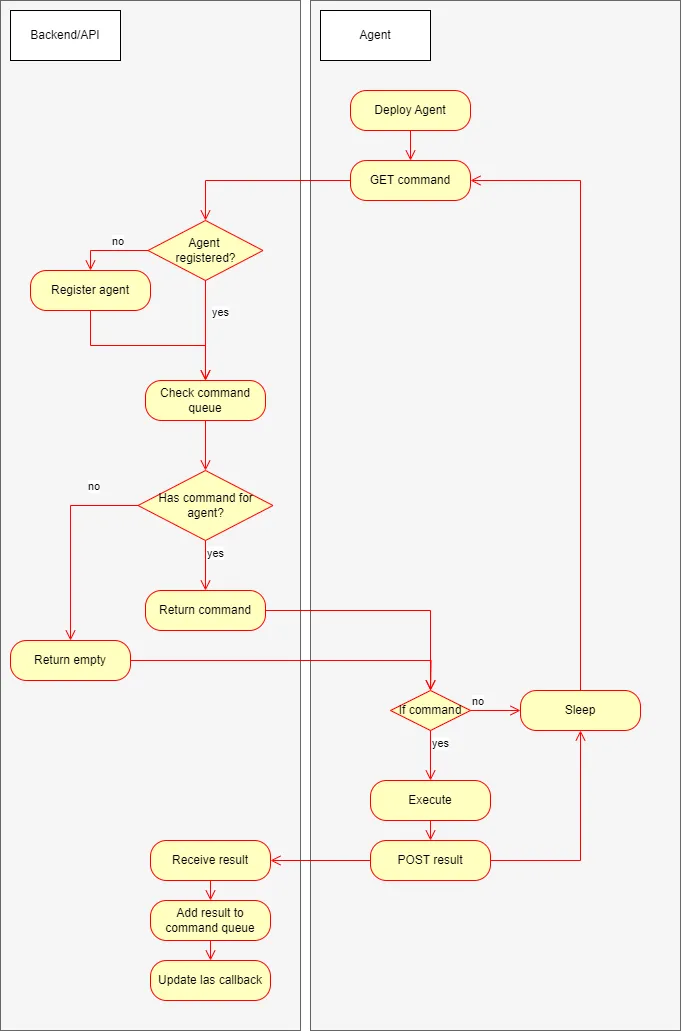
\includegraphics[width=0.8\textwidth]{includegraphics/diagramm.png} % Replace with your actual diagram file
    \caption{Process diagram of the C2 server workflow.}
    \label{fig:process_diagram}
\end{figure}

